\item \points{10} {\bf PCA} 

In class, we showed that PCA finds the ``variance maximizing'' directions onto
which to project the data.  In this problem, we find another interpretation of PCA. 

Suppose we are given a set of points $\{x^{(1)},\ldots,x^{(\nexp)}\}$. Let us
assume that we have as usual preprocessed the data to have zero-mean and unit variance
in each coordinate.  For a given unit-length vector $u$, let $f_u(x)$ be the 
projection of point $x$ onto the direction given by $u$.  I.e., if 
${\cal V} = \{\alpha u : \alpha \in \Re\}$, then 
\[
f_u(x) = \arg \min_{v\in {\cal V}} ||x-v||^2.
\]
Show that the unit-length vector $u$ that minimizes the 
mean squared error between projected points and original points corresponds
to the first principal component for the data. I.e., show that
$$ \arg \min_{u:u^Tu=1} \sum_{i=1}^\nexp \|x^{(i)}-f_u(x^{(i)})\|_2^2 \ .$$
gives the first principal component.


{\bf Remark.} If we are asked to find a $k$-dimensional subspace onto which to
project the data so as to minimize the sum of squares distance between the
original data and their projections, then we should choose the $k$-dimensional
subspace spanned by the first $k$ principal components of the data.  This problem
shows that this result holds for the case of $k=1$.

\ifnum\solutions=1 {
  \begin{answer}
After many trials, I found an instance where the algorithm is able to converge after 193 trials. 
\begin{figure}[here] %  figure placement: here, top, bottom, or page
   \centering
   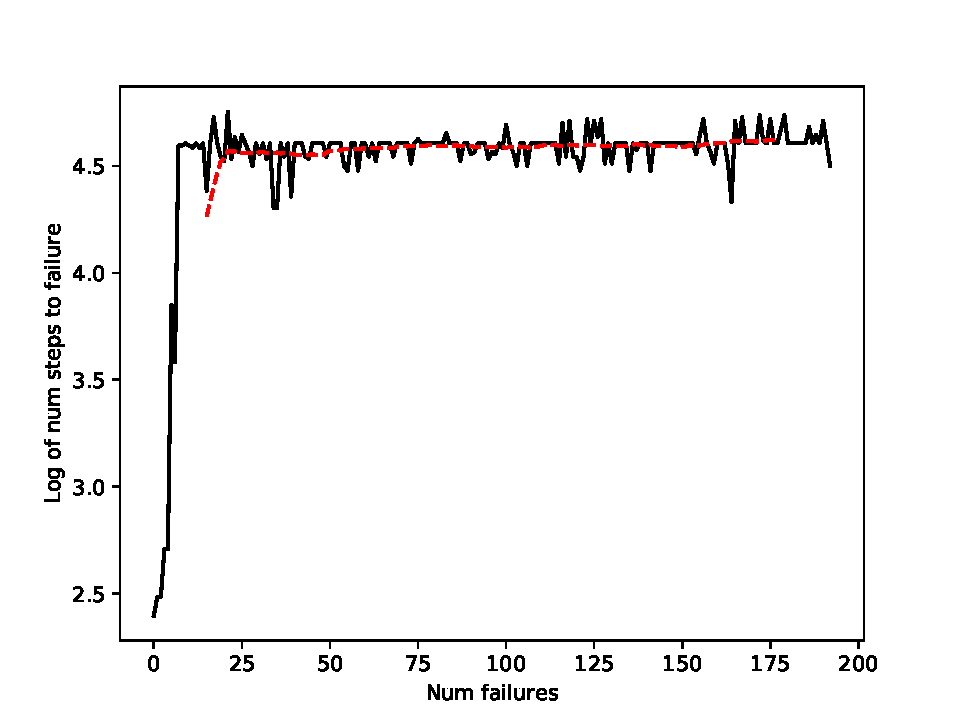
\includegraphics[width=6in]{control6.pdf} 
   \caption{Steps by Failures until Convergence}
   \label{fig:example}
\end{figure}
\end{answer}

} \fi

  
